\documentclass[12pt]{article}
\usepackage{graphicx}
\usepackage{amsmath}
\usepackage[usenames, dvipsnames]{color}
\usepackage[T1]{fontenc}
\usepackage{helvet}
\renewcommand{\rmdefault}{ptm}
\usepackage{graphicx}

\title{COP290: Complaint Management App}
\author{ Ajmeera NagaRaju (2014CS10208)\\Vipparthy Sai Esvar (2014CS10266) \\ Harshil R. Meena (2014CS10222) }

\begin{document}
\pagecolor{SpringGreen}
\maketitle



\section{Introduction}
\begin{itemize}
\item The App will have the following features (corresponding APIs would be called for their implementation):
	\begin{itemize}
		\color{blue}
		\item Login : as student or (warden/faculty or specialuser)
	\end{itemize}
\item After Login the user can:
	\begin{itemize}
		\color{blue}
		\item View the list of complaints related to the user
		\item View the list of notifications
		\item Lodge a new complaint
		\item Mark their vote on a common complaint
		\item Mark the complaints in their jurisdiction as resolved
		\item Logout
	\end{itemize}
\item Also, the specialuser can:
	\begin{itemize}
		\color{blue}
		\item Add any new user to the database
	\end{itemize}
\item We will be using a public Web2Py server coded in Python for our application
\item We have also assigned one account to the superuser who will be in-charge of adding other users. His login details are :
	\begin{itemize}
		\color{blue}
		\item Username: superuser
		\item Password: godmode
	\end{itemize}
\item The APIs will be implemented in such a manner that the assignment can be easily extended to the web clients as well
\end{itemize}

\section{User Interface}
\begin{itemize}
\item A  blank activity for the login page with two entry fields username, password and a login button
\item A navigation drawer activity for the main dashboard allowing the user the following options once he is successfully logged in:
	\begin{itemize}
		\color{blue}
		\item List of all complaints
		\item Lodge a complaint
		\item View my complaint
		\item Logout 
	\end{itemize}
 \item The fragment displaying the list of all complaints, serving as the home page when a user successfully logs in, consists of all the complaints which have been lodged by any of the users
\item On clicking up on Lodge a complaint, the user will be allowed to put up his own complaint after switching to a new activity providing the following input fields:
	\begin{itemize}
		\color{blue}
		\item Title
		\item Person to whom the complaint is addressed to
		\item Complaint Description 
		\item Complaint location and level
		\item Submit button
	\end{itemize}
\begin{figure}[ht!]
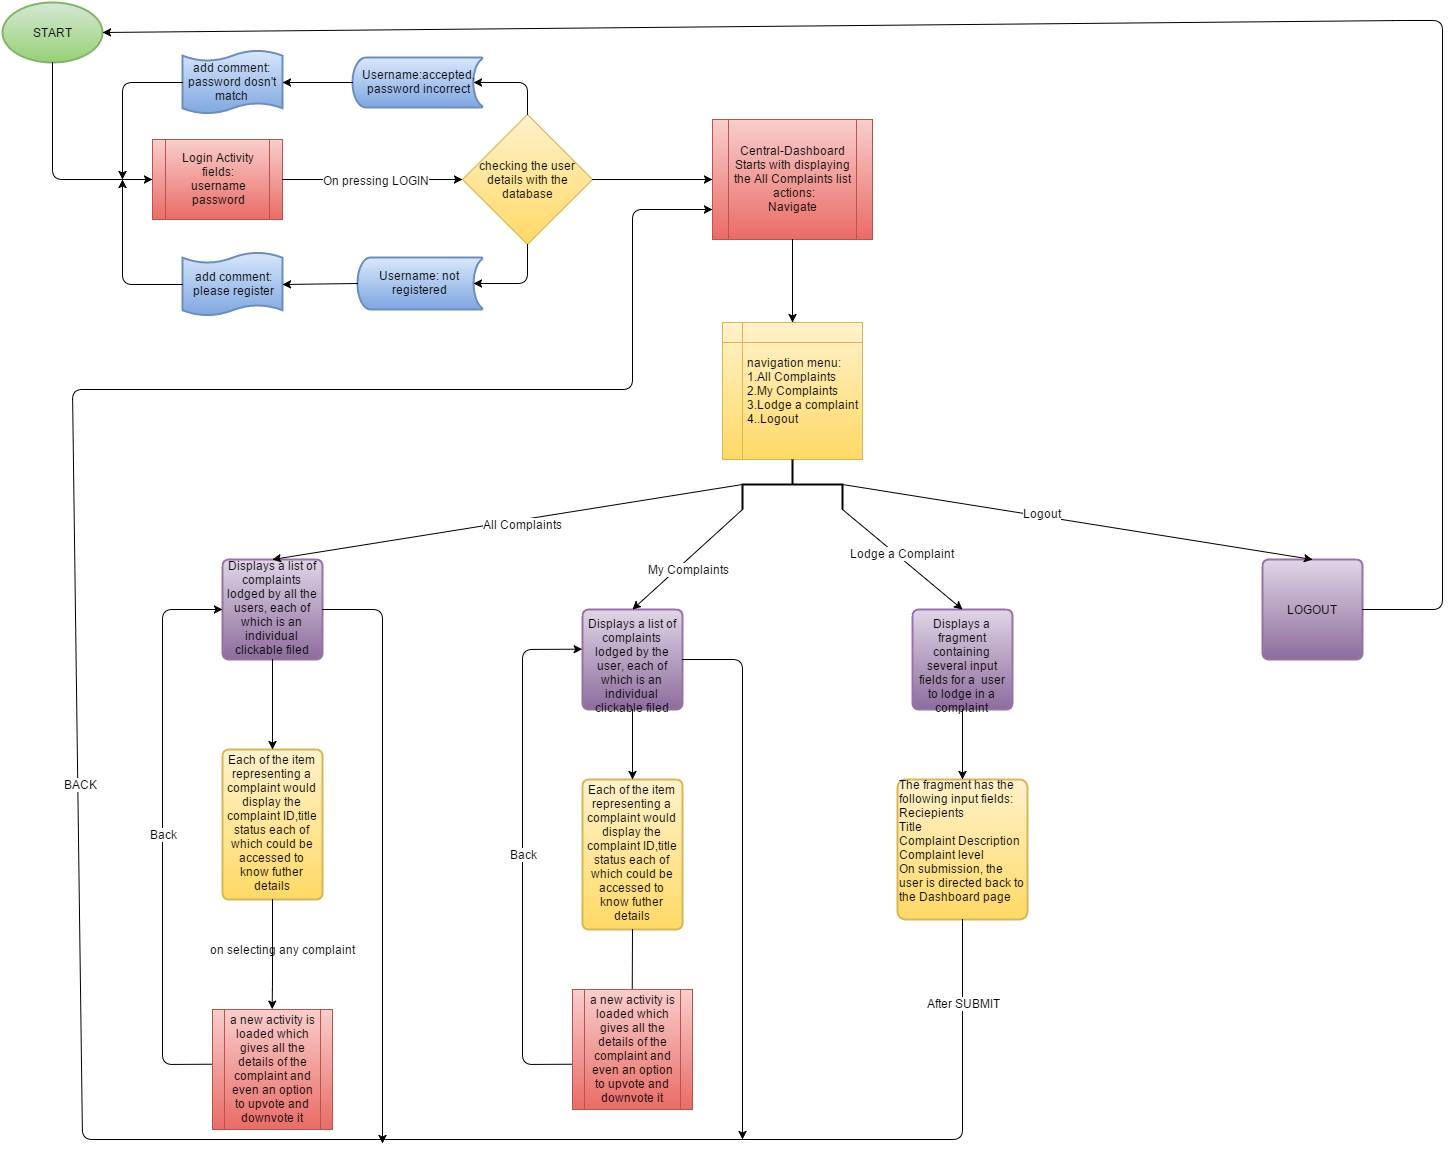
\includegraphics[width=150mm]{workflow.jpg}
\caption{Workflow \label{overflow}}
\end{figure}
\item Once a complaint is submitted, a unique complaint ID will be generated for it and the user would be given an option to either return to the home page or lodge another complaint. Also,the complaint will be displayed in the list containing all the complaints as a fragment containing the complaint ID, title, location, status, options to either upvote or downvote
\item If the user wishes to to go through the complaints lodged by him, he could choose the option from the navigation drawer which if for displaying his complaints
\item On clicking on any of these complaints, the user can see:
	\begin{itemize}
		\color{blue}
		\item Title of the complaint 
		\item Complaint ID
		\item Description of the complaint
		\item Level of complaint
		\item Number of upvotes/downvotes
		\item Also options to upvote and downvote
		\item Person to whom the complaint is addressed to
	\end{itemize}
\end{itemize}


\section{Event flow}
\begin{itemize}
\item Login:
\begin{itemize}
	\color {blue}
	\item User enters the login details on the application and presses ENTER
	\item Users details gets checked 
	\item POST request sent to the server in form of a StringRequest
	\item The server then calls the Login API with the form data
	\item The API checks if the login details are present in the database by fetching the content using SQLite
	\item If the content is present in the tables then the Dashboard for the user gets shown
\end{itemize}
\begin{figure}[ht!]
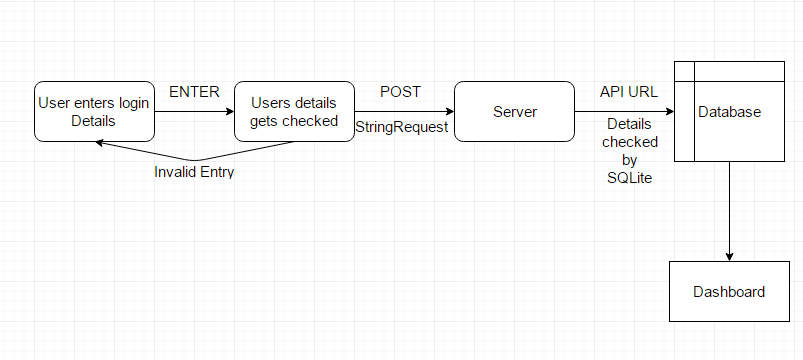
\includegraphics[width=150mm]{eventflow.png}
\caption{Sample event flow \label{overflow}}
\end{figure}
\item Logout:
\begin{itemize}
	\color {blue}
	\item User presses the LOGOUT button
	\item GET request sent to the server in form of a StringRequest
	\item The server then calls the Logout API url
	\item The user gets redirected to the Login screen
\end{itemize}
\item Notifications:
\begin{itemize}
	\color {blue}
	\item User presses the NOTIFICATIONS button
	\item GET request sent to the server in form of a StringRequest
	\item The server then calls the Notifications API url
	\item The API fetches all the data from the Notifications Table using SQLite and sets it as the input for the ListView
	\item The user gets redirected to the Notifications screen
\end{itemize}
\item All complaints:
\begin{itemize}
	\color {blue}
	\item User presses the All complaints button
	\item GET request sent to the server in form of a StringRequest
	\item The server then calls the All complaints API url
	\item The API fetches all the data from the Complaints Table using SQLite and sets it as the input for the ListView
	\item The user gets redirected to the All complaints screen
\end{itemize}
\item Vote on a complaint:
\begin{itemize}
	\color {blue}
	\item User presses the Upvote/Downvote button
	\item POST request sent to the server in form of a StringRequest
	\item The server then calls the All complaints API url with the vote data
	\item The API fetches the updates the vote data of the complaint in the Complaints Table using SQLite and resets the input for the ListView
	\item All complaints screen get reloaded
\end{itemize}
\item Mark the complaint as resolved:
\begin{itemize}
	\color {blue}
	\item User presses the RESOLVED button
	\item GET request sent to the server in form of a StringRequest
	\item The server then calls the Mark the complaint as resolved API url with the complaint ID
	\item The API updates the resolved data of the corresponding complaint in the Complaints Table using SQLite and resets the input for the ListView
	\item All complaints screen gets reloaded
\end{itemize}
\item Lodge a new complaint:
\begin{itemize}
	\color {blue}
	\item User enters the complaint title and description and then presses the LODGE button
	\item POST request sent to the server in form of a StringRequest
	\item The server then calls the Lodge a new complaint API url with the complaint data
	\item The API inserts this complaint into the Complaint table using SQLite
	\item Lodge a new complaint screen get reloaded
\end{itemize}
\item Add new user to db:
\begin{itemize}
	\color {blue}
	\item superuser enters the user details and presses ENTER button
	\item POST request sent to the server in form of a StringRequest
	\item The server then calls the Add new user to db API url with the user data
	\item The API inserts this new user into the Users table using SQLite
	\item Add new user to db screen get reloaded
\end{itemize}
\end{itemize}

\begin{figure}[ht!]
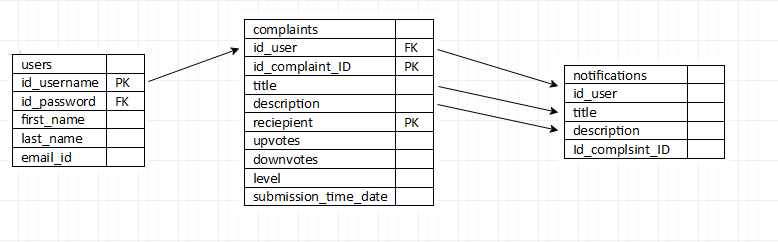
\includegraphics[width=150mm]{erd.png}
\caption{ERD \label{overflow}}
\end{figure}
\section{Data Storage}
\begin{itemize}
\item This data would be stored in a database across multiple tables (in .table format) and the database would be implemented using SQLite
\item The following tables are required :
\item Users : stores data about all the users such as 
	\begin{itemize}
		\color{blue}
		\item firstname
		\item lastname
		\item email
		\item username
		\item entryno
		\item type (0 for a student, 1 for a warden and so on)
		\item password
	\end{itemize}
\item Complaints : stores all the data for complaints
	\begin{itemize}
		\color{blue}
		\item Title
		\item Complaint ID
		\item Description
		\item Level of complaint (Individual or hostel or institute level)
		\item Number of upvotes
		\item Number of downvotes
		\item Person who lodged the complaint
		\item Person to whom the complaint is addressed to
		\item Is resolved
		\item Created at
	\end{itemize}
\item Notifications : stores all the notifications
	\begin{itemize}
		\color{blue}
		\item User ID
		\item Complaint title
		\item Complaint ID
		\item Description
		\item Is seen
		\item Created at
	\end{itemize}
\item SQLite will be used to interact between various tables (to fetch, update, insert or delete data)
\item No, the database design does not allow invalid entries, this would be ensured by type-checking the fields while defining the tables. 
\end{itemize}


\section{API's}
\begin{itemize}
\item The following is the list of APIs that will be used :
\item Login: /default/login.json?userid=<username>password=<password>
	\begin{itemize}
		\color{blue}
		\item POST request
		\item Server returns JSON response with user details and the boolean value for success
	\end{itemize}
\item Logout: /default/logout.json
	\begin{itemize}
		\color{blue}
		\item GET request
		\item Server returns JSON response with the boolean value for success
	\end{itemize}
\item Lodge new complaint: /complaints/new.jsontitle=<title>description=<desc>scope=<scope>\\assignedto=<assignedto>
	\begin{itemize}
		\color{blue}
		\item POST request
		\item Server returns JSON response with the complaint details, the users details, success and the creation time
	\end{itemize}
\item Notifications: /default/notifications.json
	\begin{itemize}
		\color{blue}
		\item GET request
		\item Server returns JSON response with a list of notification details
	\end{itemize}
\item All complaints: /default/complaints.json
	\begin{itemize}
		\color{blue}
		\item GET request
		\item Server returns JSON response with a list of complaints details alongwith the users details
	\end{itemize}
\item Vote on a complaint: /complaints/postvote.json?complaintid=<complaintid>vote=<vote>
	\begin{itemize}
		\color{blue}
		\item POST request
		\item Server returns JSON response with the complaints details alongwith the users details and a success boolean
	\end{itemize}
\item Mark the complaint as resolved: /complaints/markresolved.json?complaintid=<complaintid>
	\begin{itemize}
		\color{blue}
		\item POST request
		\item Server returns JSON response with the success boolean
	\end{itemize}
\item Add new user to db: /default/adduser.json
username=<username>password=<pass>\\firstname=<firstname>lastname=<lastname>entryno=<entryno>type=<type>
	\begin{itemize}
		\color{blue}
		\item POST request
		\item Server returns JSON response with the list of all users, the added user and the success boolean
	\end{itemize}
\end{itemize}


\section{Modularity}
\begin{itemize}
\item The project can be divided into the following modules:
	\begin{itemize}
		\color{blue}
		\item Server code
		\item Database code
		\item Android Java files for activities and other auxiliary functions
		\item User interface files
		\item Networking code
		\item Session management and cookies
		\item Google cloud messaging setup
		\item Retry policy
		\item Android client
	\end{itemize}
\end{itemize}


\section{Bug foresight}
\begin{itemize}
\item These bugs might be encountered in the project:
\begin{itemize}
	\color {blue}
	\item SQLite exceptions
	\item Heisenbergs
	\item Gradle errors
	\item Web2Py HTTP-500 (internal server) errors
	\item Missing packages
	\item Python CGI errors
	\item General and crucial interface errors
\end{itemize}
\end{itemize}


 \begin{thebibliography}{99}

\bibitem{HB98} Tutorial on setting up server: {\em
https://www.digitalocean.com/community/tutorials/how-to-use-the-web2py-framework-to-quickly-build-your-python-app}

\bibitem{CA} Design doc tips: {\em
http://www.cse.iitd.ernet.in/cs5110300/SessionAssignment2}

\end{thebibliography}

%\bibliographystyle{abbrv}
%\bibliography{references}

{\color{red} \rule{\linewidth}{0.5mm} }

\end{document}
